\documentclass{article}
\usepackage[utf8]{inputenc}
\usepackage{amsmath}
\usepackage{amssymb}
\usepackage{amsfonts}
\usepackage{amssymb}
\usepackage{minted}
\usepackage{graphicx}
\graphicspath{ {img/} }
\usepackage{titlesec}
\usepackage[a4paper,margin=1in,footskip=0.25in]{geometry}
\usepackage{fancyhdr}
\pagestyle{fancy}
%basic page layout

%draw finite state machine
\usepackage{tikz}
\usetikzlibrary{arrows,automata}
\newcommand{\hwnumber}{3}
\newcommand{\Lcvy}{\mathcal{L}}
%header and footer settings
\lhead{Algorithms and Data Structure \hwnumber}
\chead{Yiping Deng}
\rhead{\today}

\titlelabel{\thetitle\enspace}

\begin{document}
\title{Algorithms and Data Structure \hwnumber}
\author{Yiping Deng}
\maketitle
\thispagestyle{fancy}
\section*{Problem 1}
\subsection*{a)}
The implementation is included here. \\
The naive approach:
\inputminted{Python}{code/recursive_fib.py}
The bottom-up approach:
\inputminted{Python}{code/bottom_up_fib.py}
The formula approach:
\inputminted{Python}{code/formula_fib.py}
The matrix approach:
\inputminted{Python}{code/matrix_fib.py}
\subsection*{b)}
The table is here
\inputminted{Text}{code/result.txt}
and the code to generate the table
\inputminted{Python}{code/fib_timer.py}
\subsection*{c)}
The recursive approach is applying the definition, so it is correct.
The bottom up approaches maintains the loop invariant. 
Before and after the loop, the Fibonacci number n1 and n2 is maintained.
They are adjacent Fibonacci number.
The formula can be validated using induction.
The last formula, similar to the previous one, is using the same induction technique.
A quick check of the proof will be via a unit test. 
In the above code, you can see the unit test is running correctly.
The unit test is in the calculate function. You can run it by
doing \textbf{python -m doctest -v fib\_timer.py}
\subsection*{d)}
recursive approach \\
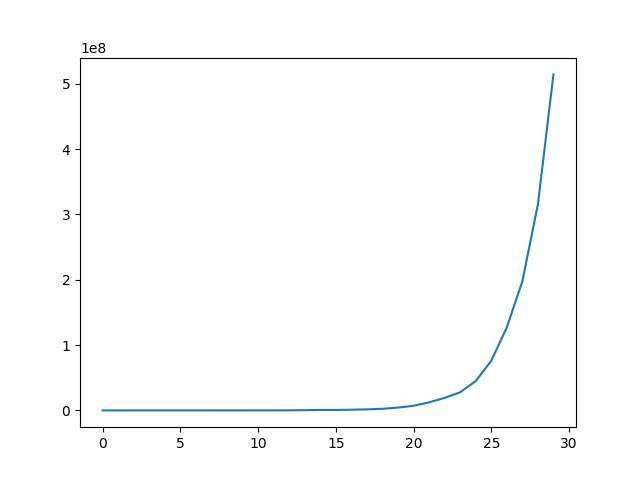
\includegraphics{recursive.png}
bottom up approach \\
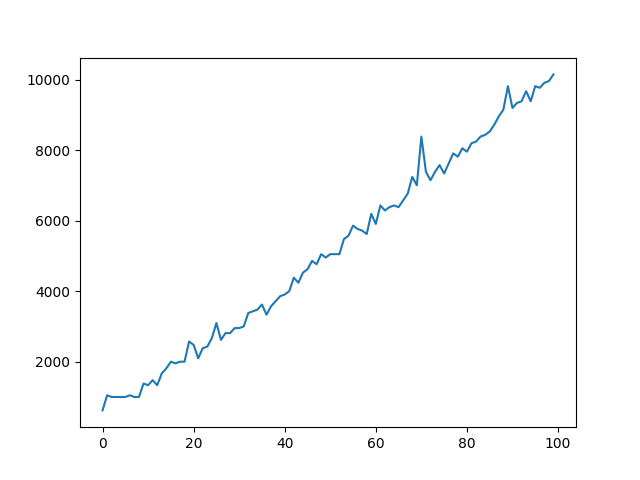
\includegraphics{bottom_up.png}
formula approach \\
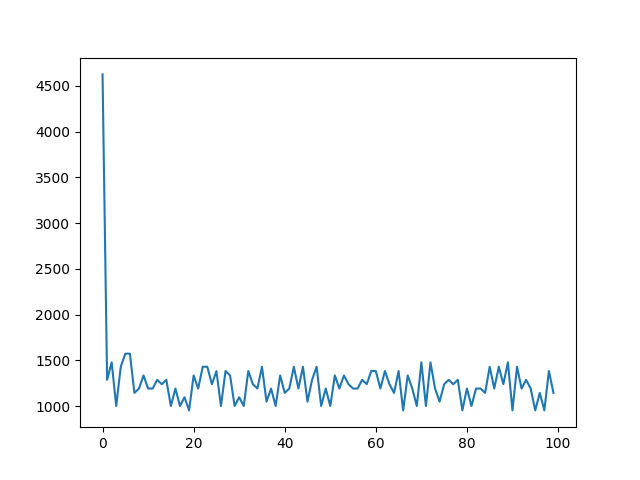
\includegraphics{formula.png}
matrix approach \\
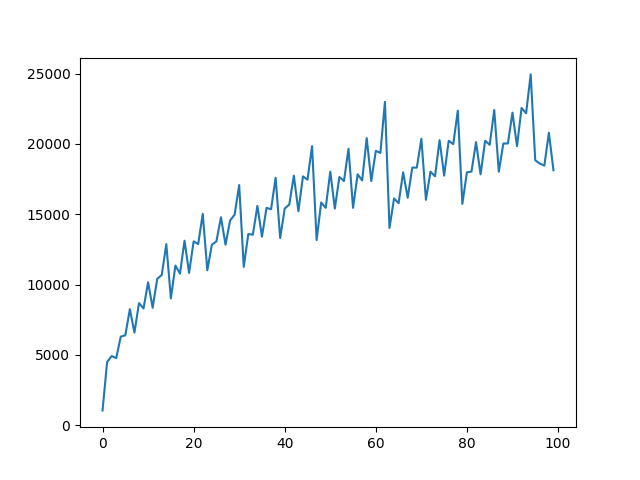
\includegraphics{matrix.png}
the log-log plot \\
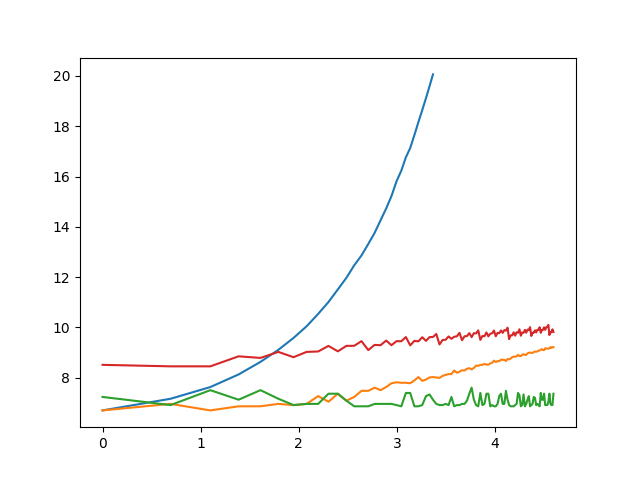
\includegraphics{loglog.png}
\section*{Problem 2}
\subsection*{a)}
The time complexity of addition of arbitrary length $n$ array
is $O(n)$, and also, the brute force approach will add for $2^n$ times.
In total, it is $O(n * 2^n) = O(2^n)$
A smarter approach is using the algorithm below.
\begin{minted}{Python}
def mul(x, y):
    if x == 1:
        return y
    halved = mul(x // 2, y)

    res = halved << 1
    # bit shift 1 to double the value,
    # this operation is linear time in modern CPU

    if x % 2 == 1;
        res = res + y
        # this operation is in linear time
    return res
\end{minted}
As you can see in this algorithm, use implement it by
calculate the half value first, and sum it up. The total
running time for this naive approach is $O(n^2)$
\subsection*{b)}
Using Gaussian approach, the algorithm is below
\inputminted{Python}{algo.py}
It uses the formula:
\begin{align*}
    xy &= (2^{n/2}  x_l + x_r)(2^{n/2} y_l + y_r) = 2^n x_l y_l + 2^{n/2}(x_l y_r + x_r y_l) + x_r y_r \\
    x_l y_r + x_r y_l &= (x_l + x_r)(y_l + y_r) - x_l y_l -x_r y_r
\end{align*}

\subsection*{c)}
The recurrence is clearly
$$ T(n) = 3T(n / 2) + O(n) $$
because addition is linear, and the recursive call reduce the size by half.
\subsection*{d)}
Using the tree method, the depth is $log_2 n$, and at the bottom
level, it is $O(3^{log_2 n})$ operation. Such sum is a geometric series, bounded above by a the highest term
by a constant factor. Thus, it is $O(3^{log_2 n}) = O(n^{log_2 3})$ \\
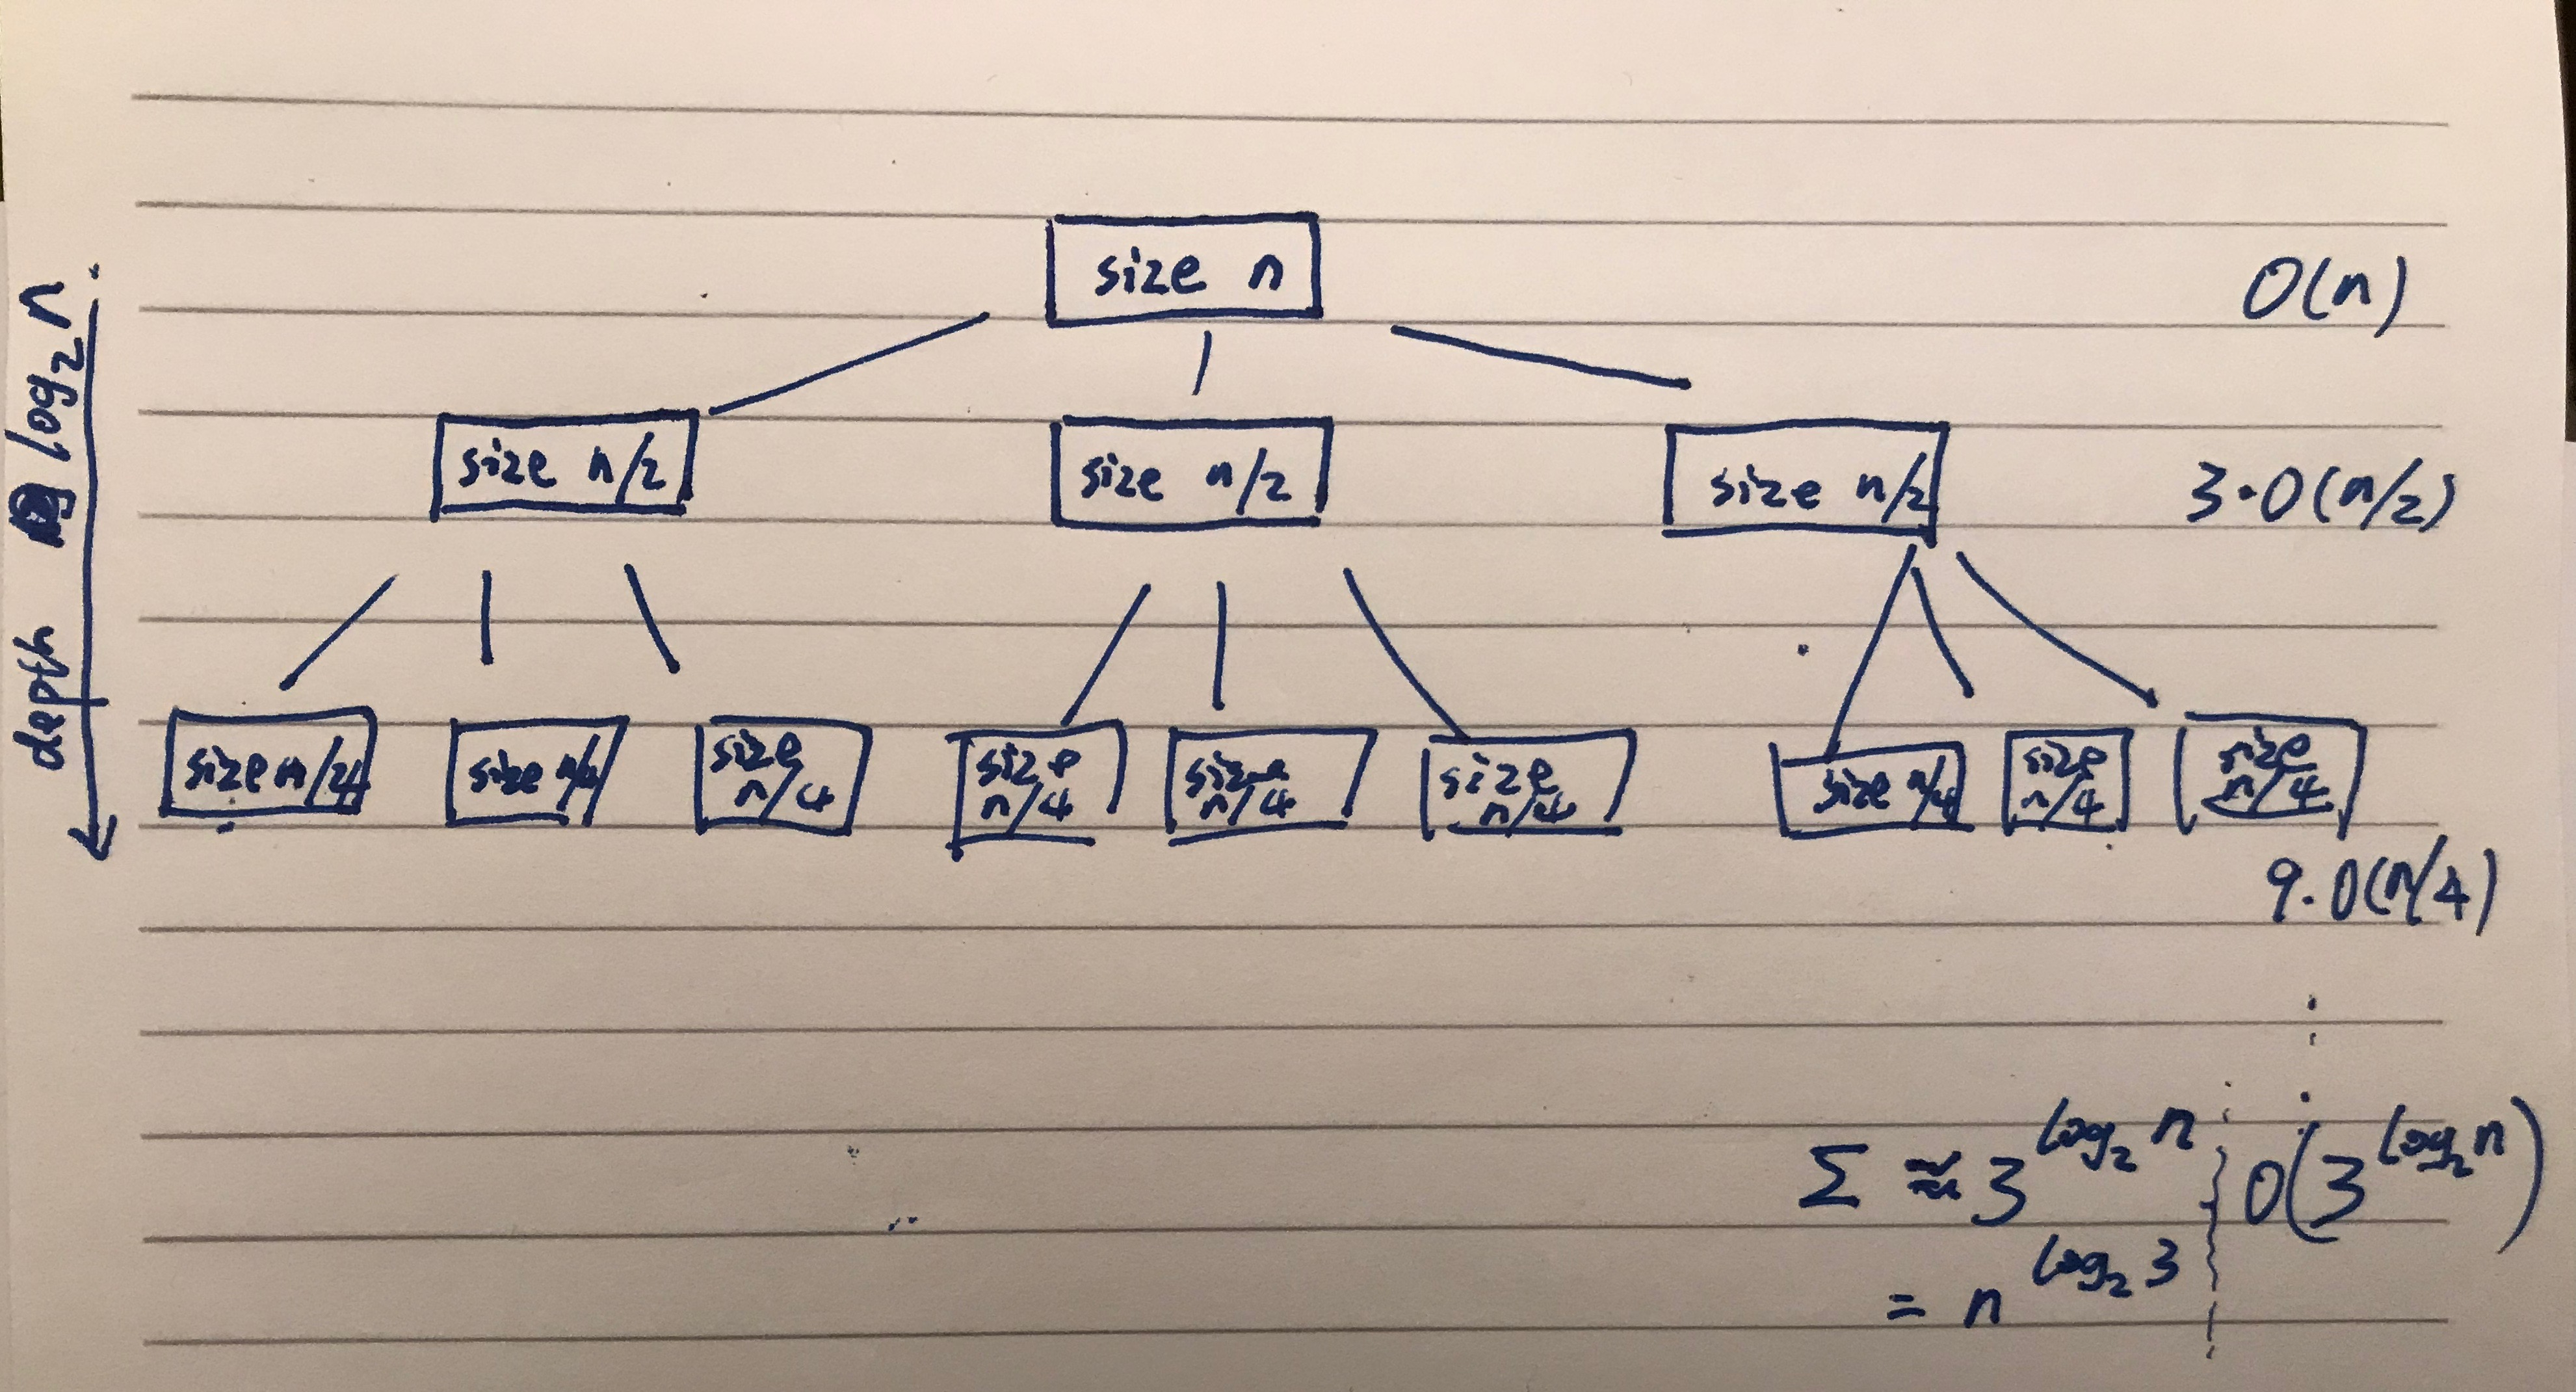
\includegraphics[width=\textwidth,height=\textheight,keepaspectratio]{tree.jpg}
\subsection*{e)}
Using the master theorem, 
$a = 3$, $b = 2$, $d = 1$, thus $T(n) = O(n^{log_2 3})$
\end{document}
